\documentclass[report.tex]{subfiles}
\begin{document}
\subsection{Results}
This section displays the results of the experiments described in section \ref{sec:Lab1 methodology}.

\subsubsection{Microstrip Parameters}
The result of this experiment is given in Table \ref{table: Lab1 Simulated Microstrip parameters}.

\begin{table}[h]
    \centering
    \caption{Simulated microstrip parameters.\label{table: Lab1 Simulated Microstrip parameters}}
    \begin{tabular}{c | c | c | c}
        $w [\text{mm}]$ & $l [\text{mm}]$ & $\epsilon_{eff}$ & $\lambda [\text{mm}]$\\
        \hline
		2.38 & 149.83 & 1.89 & 217.7
    \end{tabular}
\end{table}

\subsubsection{Signal Propagation Delay}\label{subsubsec:Lab 1 Signal propagation delay}

The propagation speed given in Figure \ref{fig:Lab1 propagation speed} corresponds to 65 \% of the speed of light and the resulting formula for the signal propagation delay, rewritten from \ref{eq: Lab1 propagation delay}, is given as

\begin{equation}
	\Delta t_p = \dfrac{100}{65 c}l.
\end{equation}

\vspace*{\fill}

\begin{figure}[h]
    \centering
	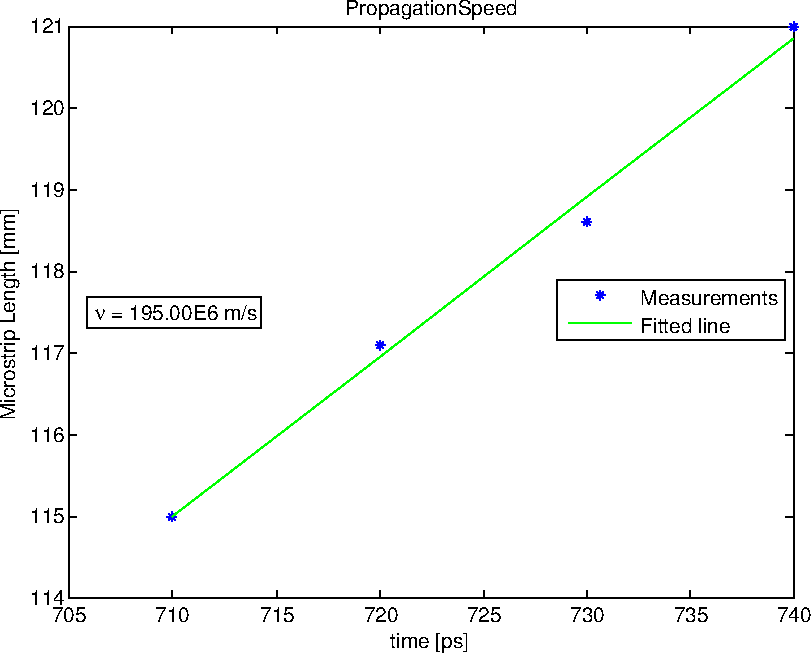
\includegraphics[scale=0.9]{propagation_speed}
	\caption{Propagation speed}
	\label{fig:Lab1 propagation speed}
\end{figure}

\vspace*{\fill}

\clearpage

\subsubsection{Reflection Coefficient}\label{subsubsec:Lab1 ref coeff}

\begin{figure}[H]
    \centering
	\subfloat[$0\:\Omega$]{
    	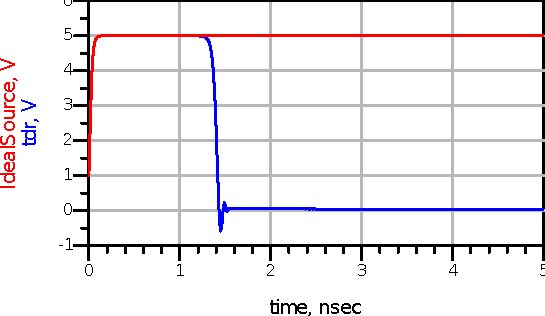
\includegraphics[scale=0.65]{0Ohm}
    }
    \subfloat[$25\:\Omega$]{
        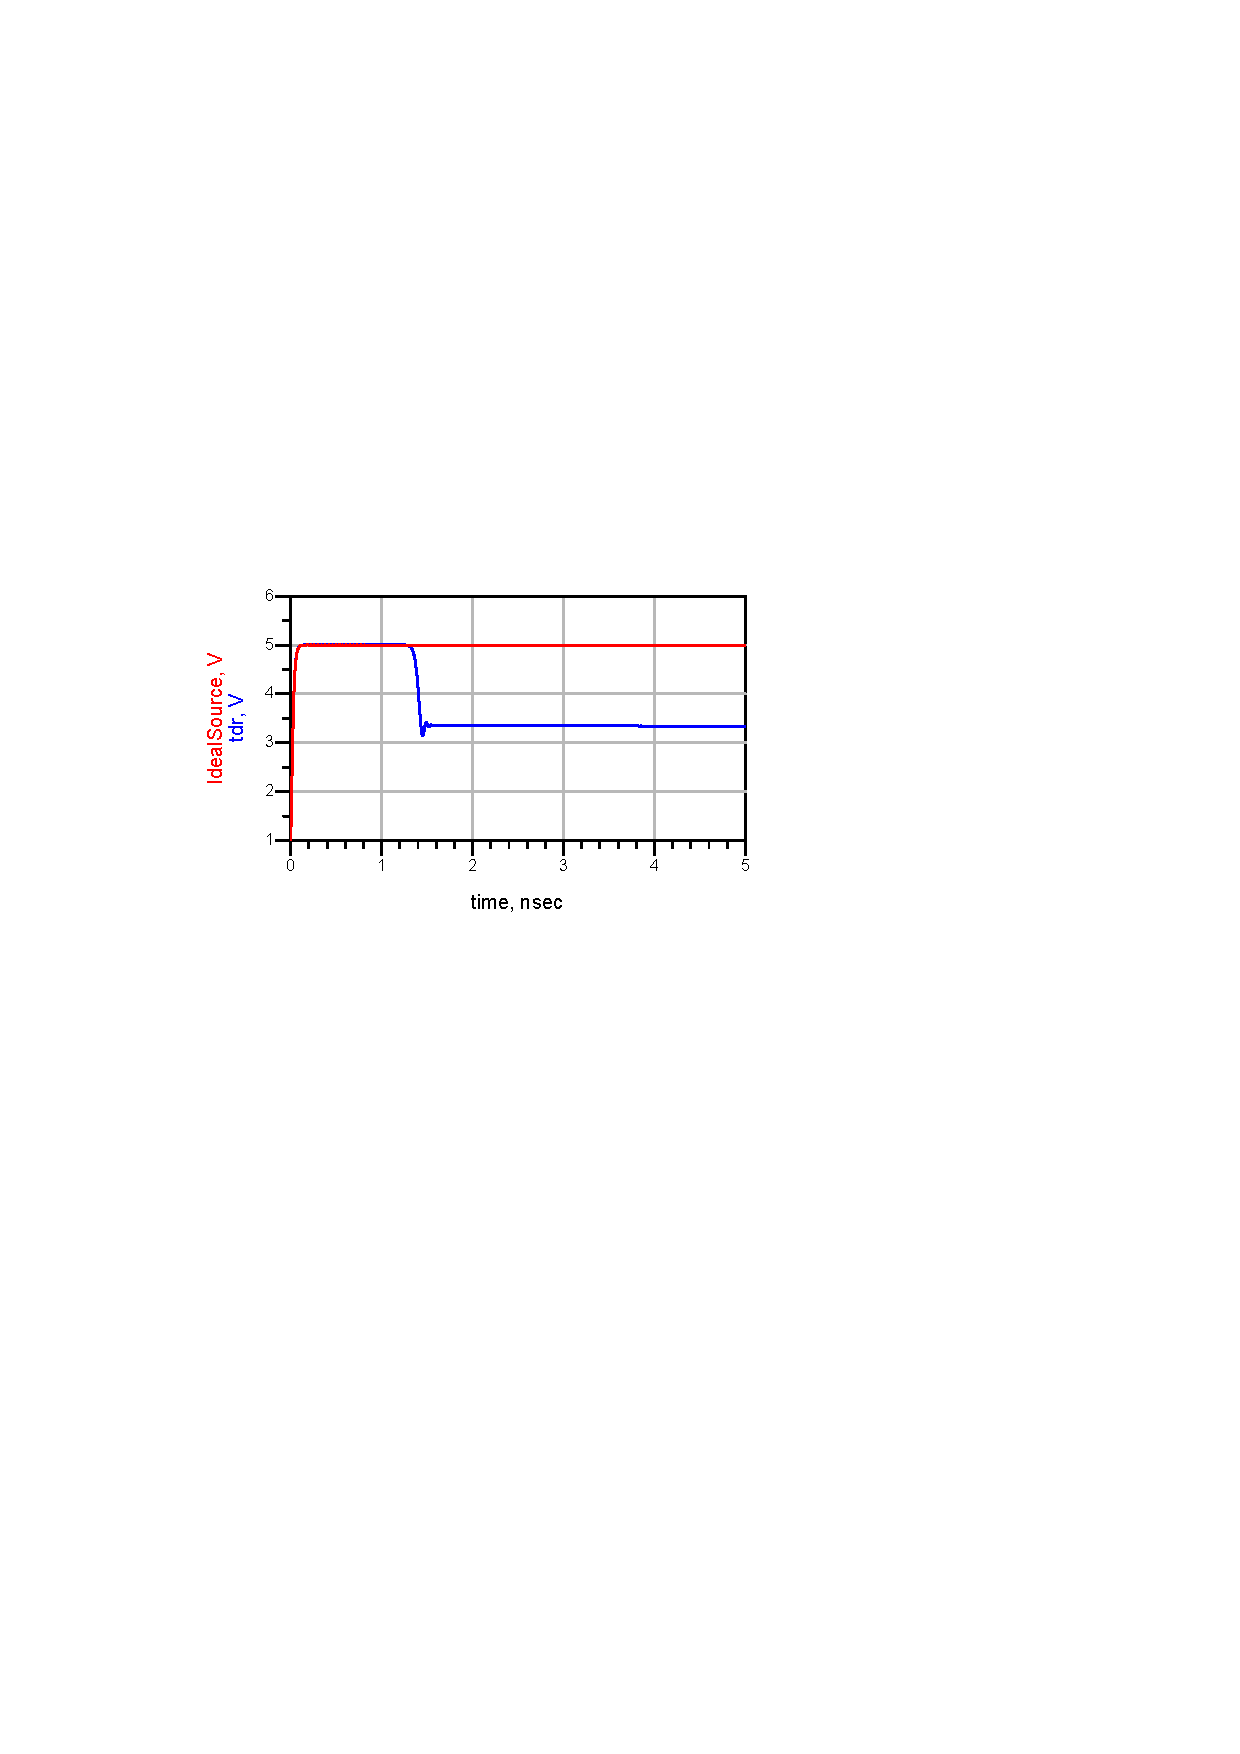
\includegraphics[scale=0.65]{25Ohm}
    }
    
    \subfloat[$100\:\Omega$]{
        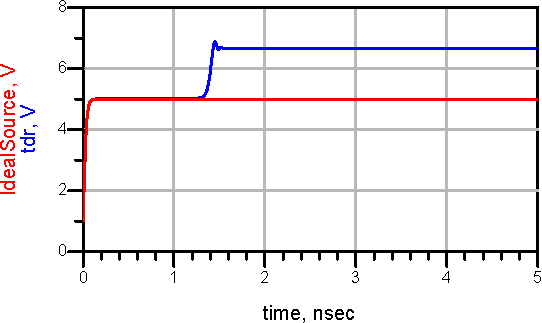
\includegraphics[scale=0.65]{100Ohm}
    }
    \subfloat[$1\:\text{M}\Omega$]{
        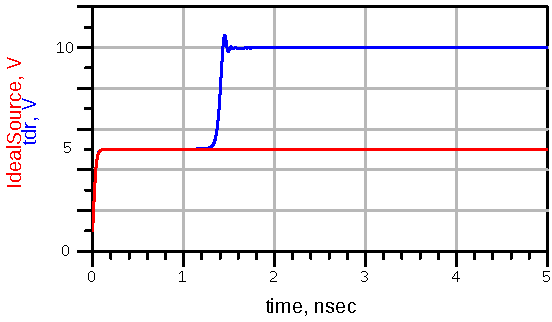
\includegraphics[scale=0.65]{1000000}
    }
	\caption{Voltage recorded at the output of reflection coefficient experiment.}
	\label{fig:Lab 1 Voltage recorded at the output.}
\end{figure}

The red lines in Figure \ref{fig:Lab 1 Voltage recorded at the output.} shows the incident wave and the blue lines depicts the voltage recorded at the output.

\subsubsection{Transmission Line as Load}
The following figure show how the output response relates to the termination.

\begin{figure}[H]
	\centering
	\subfloat[$\lambda$]{
        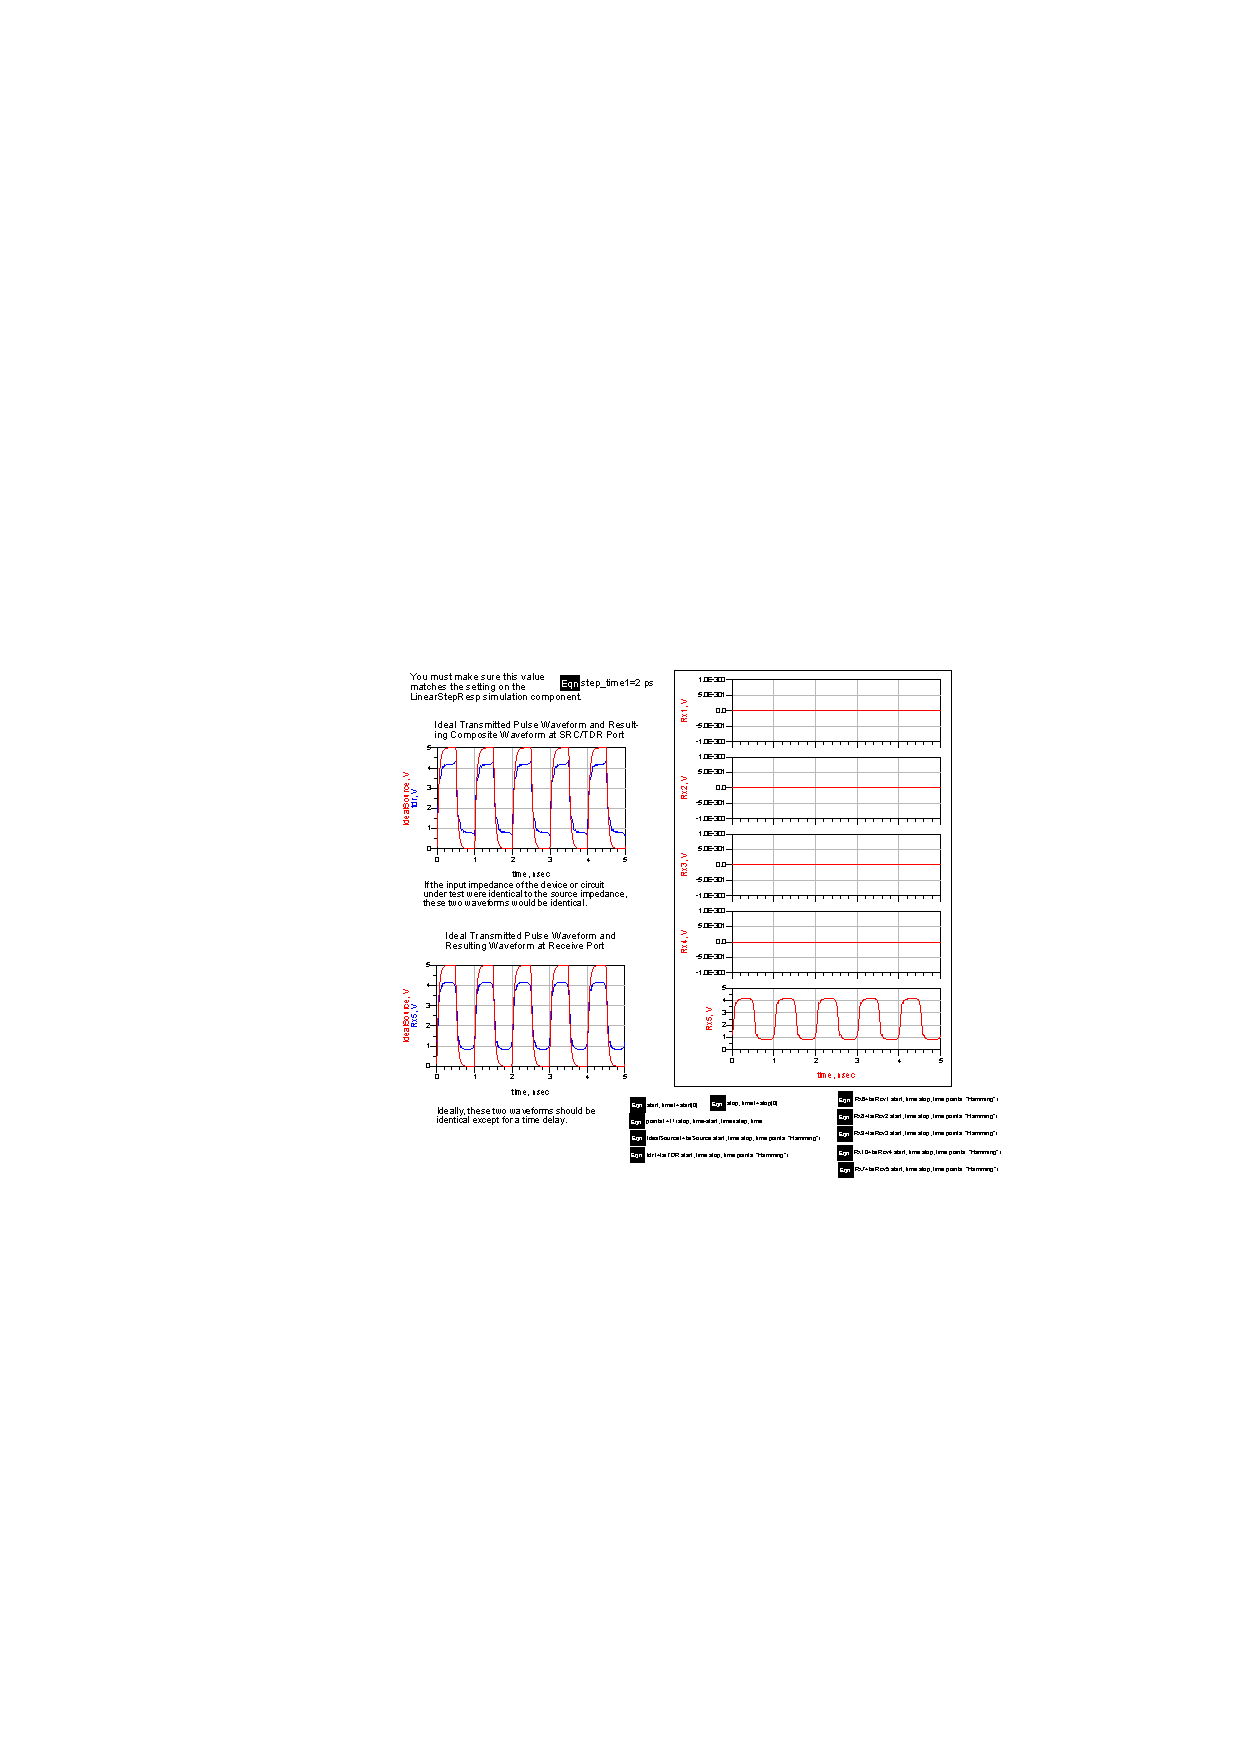
\includegraphics[scale=1]{lambda}
	}
	\subfloat[$\sfrac{\lambda}{4}$]{
    	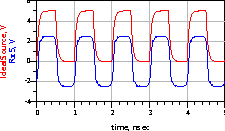
\includegraphics[scale=1]{lambda_4}
    }
    \subfloat[$\sfrac{\lambda}{8}$]{
        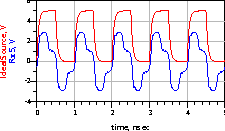
\includegraphics[scale=1]{lambda_8}
    }
	\caption{Pulse response with different transmission line terminations.}
	\label{fig:Lab 1 Pulse responses.}
\end{figure}

\end{document}